\chapter{Stand der Technik}
\label{cha:Stand der Technik}

\section{ERP: Definition und Übersicht}
\label{sec:ERP: Definition und Übersicht}
ERP Systeme sind umfangreiche kommerzielle Softwaresysteme, mit der Kernaufgabe, alle Abteilungen und Prozesse eines Unternehmens soweit wie möglich digital abzubilden\cite{doi:10.1002/smr.239}. Ein ERP-System stellt für ein Unternehmen somit eine zentrale Verarbeitungs- und Datensicherungsplattform für sämtliche unternehmensrelevanten Geschäftsdaten bereit. Die Daten sind hierbei in einem einzelnem System erfasst, und sind so sofort für alle Unternehmensbereiche verfügbar. Es sind keine Synchronisierungsschritte oder Schnittstellen innerhalb des Systems nötig. Durch die zentrale Datenerfassung, stellt ein ERP-System eine durchgängige Informationsquelle für alle Unternehmensbereiche dar, die bei der Prozessanalyse und Analyse als Datenbasis für geschäftliche Entscheidungsträger unabdingbar ist.

Im Gegensatz zu abteilungsbezogenen Systemstrukturen (Insellösungen) ist es durch Einsatz eines ERP-Systems möglich Funktionen zu nutzen, für deren Durchführung Informationen aus mehreren Abteilungen nötig sind\cite{DynamicsNAV2018Anwenderbuch}. So kann zum Beispiel bei Eingang eines Auftrags sofort automatisiert geprüft werden, ob der Auftrag angenommen werden soll. Entscheidungen wie diese basieren auf einem sehr breiten Datenstamm aus den verschiedenen Abteilungen. Aus den Daten der Finanzabteilung können Zahlungsmoral, offene Beträge des Kunden und ein voraussichtlicher Deckungsbeitrag eine Rolle für diese Entscheidung spielen. Anhand der Lagerhaltungsdaten kann sofort eine Verfügbarkeitsprüfung für die bestellten Artikel durchgeführt werden. Mithilfe von Produktions- und Personaldaten wird ausgewertet, ob ausreichend Personal und Maschinenressourcen für die Erfüllung des Auftrags zur Verfügung stehen. Dies sind nur einige wenige Beispiele, wie ein ERP-System bei der täglichen unternehmerischen Tätigkeit behilflich sein kann.

Da in ERP-Systemen der Zugriff auf die Datenbank nicht durch die Systemarchitektur eingeschränkt ist, muss der Zugang zu den Daten im System über ein Rechte- und Modulsystem gesteuert werden\cite{DynamicsNAV2018Anwenderbuch}. Berechtigungssätze lassen sich hier meist sehr feingranular definieren, sodass einerseits der Schutz sensibler Daten gewährleistet ist, jedoch andererseits alle benötigten Daten entsprechend betrachtet und verarbeitet werden können.

\pagebreak

\begin{figure}[h]
	\centering
	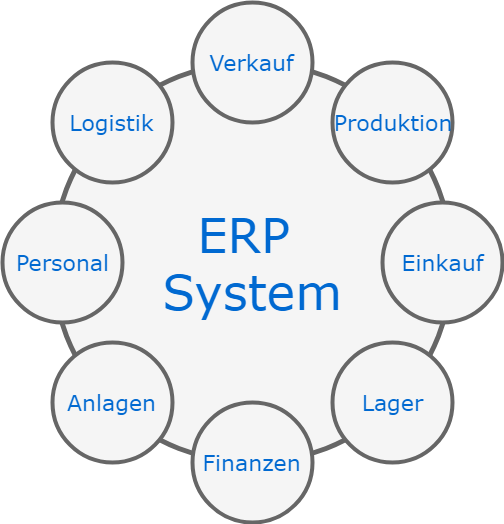
\includegraphics[width=70mm]{images/ERPModules.png}
	\caption{Schematische Darstellung: Modularisierung anhand Unternehmensabteilung}
	\label{fig:Modulisierung}
\end{figure}

Um die umfangreichen Funktionalitäten eines ERP-Systems zu gliedern und aufzuteilen, bedienen sich die meisten Hersteller eines Modul-Systems. Meist spiegelt die Aufteilung dieser Module die einzelnen Abteilungen eines Unternehmens wieder. So verteilt sich die Gesamtfunktionalität eines Systems beispielsweise auf ein Einkaufsmodul, ein Vertriebsmodul und viele andere Teilbereichsmodule auf. 
Diese Module können in ihren Grundzügen unabhängig voneinander verwendet werden. So kann ein Unternehmen beispielsweise entscheiden, vorerst nur Finanzen und Personal über das System zu verwalten. Andere Module können im Laufe der Zeit stückweise in Betrieb genommen werden. Zu den bekanntesten ERP Herstellern zählen unter anderen IBM, SAP, Microsoft, Infor und Sage.

\pagebreak
\section{Geschichte und Grundarchitektur Dynamics 365 Business Central}
\label{sec:Grundarchitektur Dynamics 365 Business Central}

\subsection{Geschichte}
\label{subsec:Geschichte}
Das ERP-System, dass heute \textit{Microsoft Dynamics 365 Business Central} heißt, erschien ursprünglich 1984 unter dem Namen \textit{PCPlus} als ein ERP System für Microsoft DOS in Dänemark\cite{DesignAndImplementationGayer}. Während seiner mittlerweile 35-jährigen Geschichte wurde das Produkt einige Male neu benannt und an den technischen Fortschritt angepasst. Was 1984 begann, wurde 1995 unter dem Namen \textit{Navision Financials} als das erste ERP-Produkt mit grafischer Benutzeroberfläche für Windows95 präsentiert. 2002 wurde \textit{Navision Financials} von Microsoft gekauft und unter dem Namen \textit{Microsoft Business Solutions Navision} vertrieben. In all diesen Jahren basierte die Datenspeicherung des Systems in einem komplexen Dateibasierten Format. Im Jahr 2008 passiert dann der Schritt zu Microsoft SQL Server und der 3-Schichten-Architektur, nun unter dem Namen \textit{Microsoft Dynamics NAV 2009}. Der vorerst letzte Meilenstein in der Geschichte des Systems ist 2018. Das System wird nun als Cloud-ERP-System unter dem Namen \textit{Microsoft Dynamics 365 Business Central} betrieben.

Trotz den vielen Versionen und der jahrzehntelangen Geschichte dieses Systems, finden sich auch in der heutigen Code-Basis noch viele Passagen, die bereits in den 1980er Jahren entstanden, und bis heute produktiv eingesetzt werden.

\subsection{3-Schichten Architektur}
\label{subsec:3-Schichten Architektur}
Dynamics 365 Business Central basiert auf einer 3-Schichten Architektur. Durch Schichtenarchitekturen lassen sich die Aufgabengebiete bzw. Teile eines komplexen Softwaresystems aufteilen. Im Falle von Dynamics Business Central 365 unterscheiden wir zwischen der Endbenutzerschicht, der Serverschicht und der Datenbankschicht.

\begin{figure}[h]
	\centering
	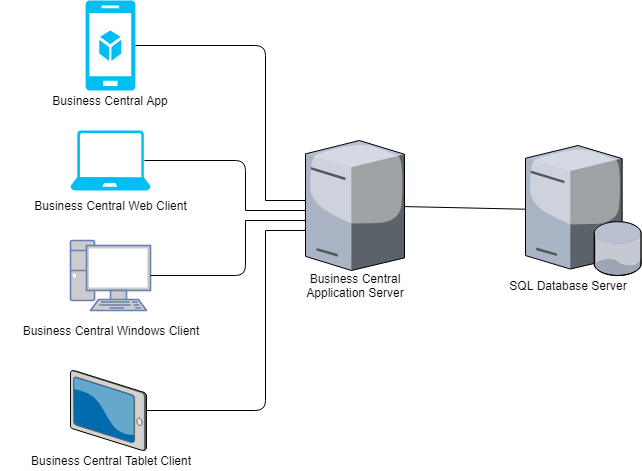
\includegraphics[width=100mm]{images/3TierArchitecture.png}
	\caption{Dynamics 365 Business Central: 3-Schichten Architektur}
	\label{fig:Image3TierArchitecture}
\end{figure}


\pagebreak
\section{Objektarten in Business Central}
\label{sec:Objektarten in Business Central}